% Options for packages loaded elsewhere
\PassOptionsToPackage{unicode}{hyperref}
\PassOptionsToPackage{hyphens}{url}
\PassOptionsToPackage{dvipsnames,svgnames,x11names}{xcolor}
%
\documentclass[
  letterpaper,
  DIV=11,
  numbers=noendperiod]{scrartcl}

\usepackage{amsmath,amssymb}
\usepackage{iftex}
\ifPDFTeX
  \usepackage[T1]{fontenc}
  \usepackage[utf8]{inputenc}
  \usepackage{textcomp} % provide euro and other symbols
\else % if luatex or xetex
  \usepackage{unicode-math}
  \defaultfontfeatures{Scale=MatchLowercase}
  \defaultfontfeatures[\rmfamily]{Ligatures=TeX,Scale=1}
\fi
\usepackage{lmodern}
\ifPDFTeX\else  
    % xetex/luatex font selection
\fi
% Use upquote if available, for straight quotes in verbatim environments
\IfFileExists{upquote.sty}{\usepackage{upquote}}{}
\IfFileExists{microtype.sty}{% use microtype if available
  \usepackage[]{microtype}
  \UseMicrotypeSet[protrusion]{basicmath} % disable protrusion for tt fonts
}{}
\makeatletter
\@ifundefined{KOMAClassName}{% if non-KOMA class
  \IfFileExists{parskip.sty}{%
    \usepackage{parskip}
  }{% else
    \setlength{\parindent}{0pt}
    \setlength{\parskip}{6pt plus 2pt minus 1pt}}
}{% if KOMA class
  \KOMAoptions{parskip=half}}
\makeatother
\usepackage{xcolor}
\setlength{\emergencystretch}{3em} % prevent overfull lines
\setcounter{secnumdepth}{-\maxdimen} % remove section numbering
% Make \paragraph and \subparagraph free-standing
\ifx\paragraph\undefined\else
  \let\oldparagraph\paragraph
  \renewcommand{\paragraph}[1]{\oldparagraph{#1}\mbox{}}
\fi
\ifx\subparagraph\undefined\else
  \let\oldsubparagraph\subparagraph
  \renewcommand{\subparagraph}[1]{\oldsubparagraph{#1}\mbox{}}
\fi


\providecommand{\tightlist}{%
  \setlength{\itemsep}{0pt}\setlength{\parskip}{0pt}}\usepackage{longtable,booktabs,array}
\usepackage{calc} % for calculating minipage widths
% Correct order of tables after \paragraph or \subparagraph
\usepackage{etoolbox}
\makeatletter
\patchcmd\longtable{\par}{\if@noskipsec\mbox{}\fi\par}{}{}
\makeatother
% Allow footnotes in longtable head/foot
\IfFileExists{footnotehyper.sty}{\usepackage{footnotehyper}}{\usepackage{footnote}}
\makesavenoteenv{longtable}
\usepackage{graphicx}
\makeatletter
\def\maxwidth{\ifdim\Gin@nat@width>\linewidth\linewidth\else\Gin@nat@width\fi}
\def\maxheight{\ifdim\Gin@nat@height>\textheight\textheight\else\Gin@nat@height\fi}
\makeatother
% Scale images if necessary, so that they will not overflow the page
% margins by default, and it is still possible to overwrite the defaults
% using explicit options in \includegraphics[width, height, ...]{}
\setkeys{Gin}{width=\maxwidth,height=\maxheight,keepaspectratio}
% Set default figure placement to htbp
\makeatletter
\def\fps@figure{htbp}
\makeatother

\KOMAoption{captions}{tableheading}
\makeatletter
\makeatother
\makeatletter
\makeatother
\makeatletter
\@ifpackageloaded{caption}{}{\usepackage{caption}}
\AtBeginDocument{%
\ifdefined\contentsname
  \renewcommand*\contentsname{Table of contents}
\else
  \newcommand\contentsname{Table of contents}
\fi
\ifdefined\listfigurename
  \renewcommand*\listfigurename{List of Figures}
\else
  \newcommand\listfigurename{List of Figures}
\fi
\ifdefined\listtablename
  \renewcommand*\listtablename{List of Tables}
\else
  \newcommand\listtablename{List of Tables}
\fi
\ifdefined\figurename
  \renewcommand*\figurename{Figure}
\else
  \newcommand\figurename{Figure}
\fi
\ifdefined\tablename
  \renewcommand*\tablename{Table}
\else
  \newcommand\tablename{Table}
\fi
}
\@ifpackageloaded{float}{}{\usepackage{float}}
\floatstyle{ruled}
\@ifundefined{c@chapter}{\newfloat{codelisting}{h}{lop}}{\newfloat{codelisting}{h}{lop}[chapter]}
\floatname{codelisting}{Listing}
\newcommand*\listoflistings{\listof{codelisting}{List of Listings}}
\makeatother
\makeatletter
\@ifpackageloaded{caption}{}{\usepackage{caption}}
\@ifpackageloaded{subcaption}{}{\usepackage{subcaption}}
\makeatother
\makeatletter
\@ifpackageloaded{tcolorbox}{}{\usepackage[skins,breakable]{tcolorbox}}
\makeatother
\makeatletter
\@ifundefined{shadecolor}{\definecolor{shadecolor}{rgb}{.97, .97, .97}}
\makeatother
\makeatletter
\makeatother
\makeatletter
\makeatother
\ifLuaTeX
  \usepackage{selnolig}  % disable illegal ligatures
\fi
\IfFileExists{bookmark.sty}{\usepackage{bookmark}}{\usepackage{hyperref}}
\IfFileExists{xurl.sty}{\usepackage{xurl}}{} % add URL line breaks if available
\urlstyle{same} % disable monospaced font for URLs
\hypersetup{
  pdftitle={Evaluacion\_crvalenz},
  pdfauthor={crvalenz},
  colorlinks=true,
  linkcolor={blue},
  filecolor={Maroon},
  citecolor={Blue},
  urlcolor={Blue},
  pdfcreator={LaTeX via pandoc}}

\title{Evaluacion\_crvalenz}
\author{crvalenz}
\date{}

\begin{document}
\maketitle
\ifdefined\Shaded\renewenvironment{Shaded}{\begin{tcolorbox}[boxrule=0pt, sharp corners, interior hidden, borderline west={3pt}{0pt}{shadecolor}, enhanced, frame hidden, breakable]}{\end{tcolorbox}}\fi

\hypertarget{protocolo-recuento-bacteriano-desde-muestras-de-contenido-intestinal}{%
\section{Protocolo recuento bacteriano desde muestras de contenido
intestinal}\label{protocolo-recuento-bacteriano-desde-muestras-de-contenido-intestinal}}

Protocolo para la obtención de recuento de bacterias recuperables, a
partir de contenido intestinal de salmon.

\hypertarget{protocolo}{%
\subsection{Protocolo}\label{protocolo}}

\begin{enumerate}
\def\labelenumi{\arabic{enumi}.}
\tightlist
\item
  Recolectar muestras de heces de salmón (21 peces) en contenedor un
  estéril (bolsa estéril tipo Whirl-Pack 13x19 cm).
\item
  Almacenar las muestras a 4°C y transportar a laboratorio.
\item
  En laboratorio, homogenizar la muestra a fin de mezclar las heces de
  los distintos peces muestreados.
\item
  Tomar entre 1 a 5 g de muestras de heces y transferir a contenedor
  estéril nuevo (tubo cónico de 15 o 50 ml dependiendo de la cantidad de
  muestra a usar).
\item
  Agregar un volumen de solución salina estéril (NaCl 0,9\%) igual a
  nueve veces el peso de la muestra (ej.: para 5 g de muestra agregar 45
  ml de Solución salina, por 4,3 g de muestra agregar 38,7 ml de
  solución salina).
\item
  Homogenizar por agitación y el contenedor con la muestra diluida. En
  este punto, la muestra se encuentra diluida diez veces (dilución -1).
\item
  Realizar 5 diluciones decimales seriadas en solución salina.
\item
  Antes de inocular las muestras, secar las placas por 15 minutos en
  condiciones de esterilidad (las placas pueden ser dejadas abiertas
  dentro de un gabinete de bioseguridad funcionando).
\item
  Con las diluciones -5, -4 y -3, inocular placas de TSA2.
\item
  Con las diluciones -5, -4 y -3, inocular placas con TSA2 con
  Florfenicol (30 µg/mL).
\item
  Con las diluciones -3, -2 y -1 inocular placas con TSA2 con
  Oxitetraciclina (30 µg/mL).
\item
  Inocular con 0,1 ml de cada dilución, en triplicado, diseminando la
  muestra con rastrillo de vidrio o asa Digralsky esterilizada
  previamente (flamear el rastrillo de vidrio con alcohol entre cada
  placa). Diseminar la muestra hasta que esta se absorba completamente
  (al absorberse la muestra observará un poco de resistencia para pasar
  el restrillo por el agar).
\item
  Cada dilución debe sembrase en triplicado en cada uno de los distintos
  medios utilizados.
\item
  Incubar las placas a 20°C por hasta 5 días, revisando el desarrollo de
  colonias diariamente.
\item
  Hacer recuento del número de colonias en aquellas placas que tengan
  entre 30 a 300 colonias, en el equipo SCAN 500, dejando registro de
  las placas procesadas.
\item
  Informar resultado en ufc/g.
\end{enumerate}

\hypertarget{esquema}{%
\subsection{Esquema}\label{esquema}}

\begin{figure}

{\centering 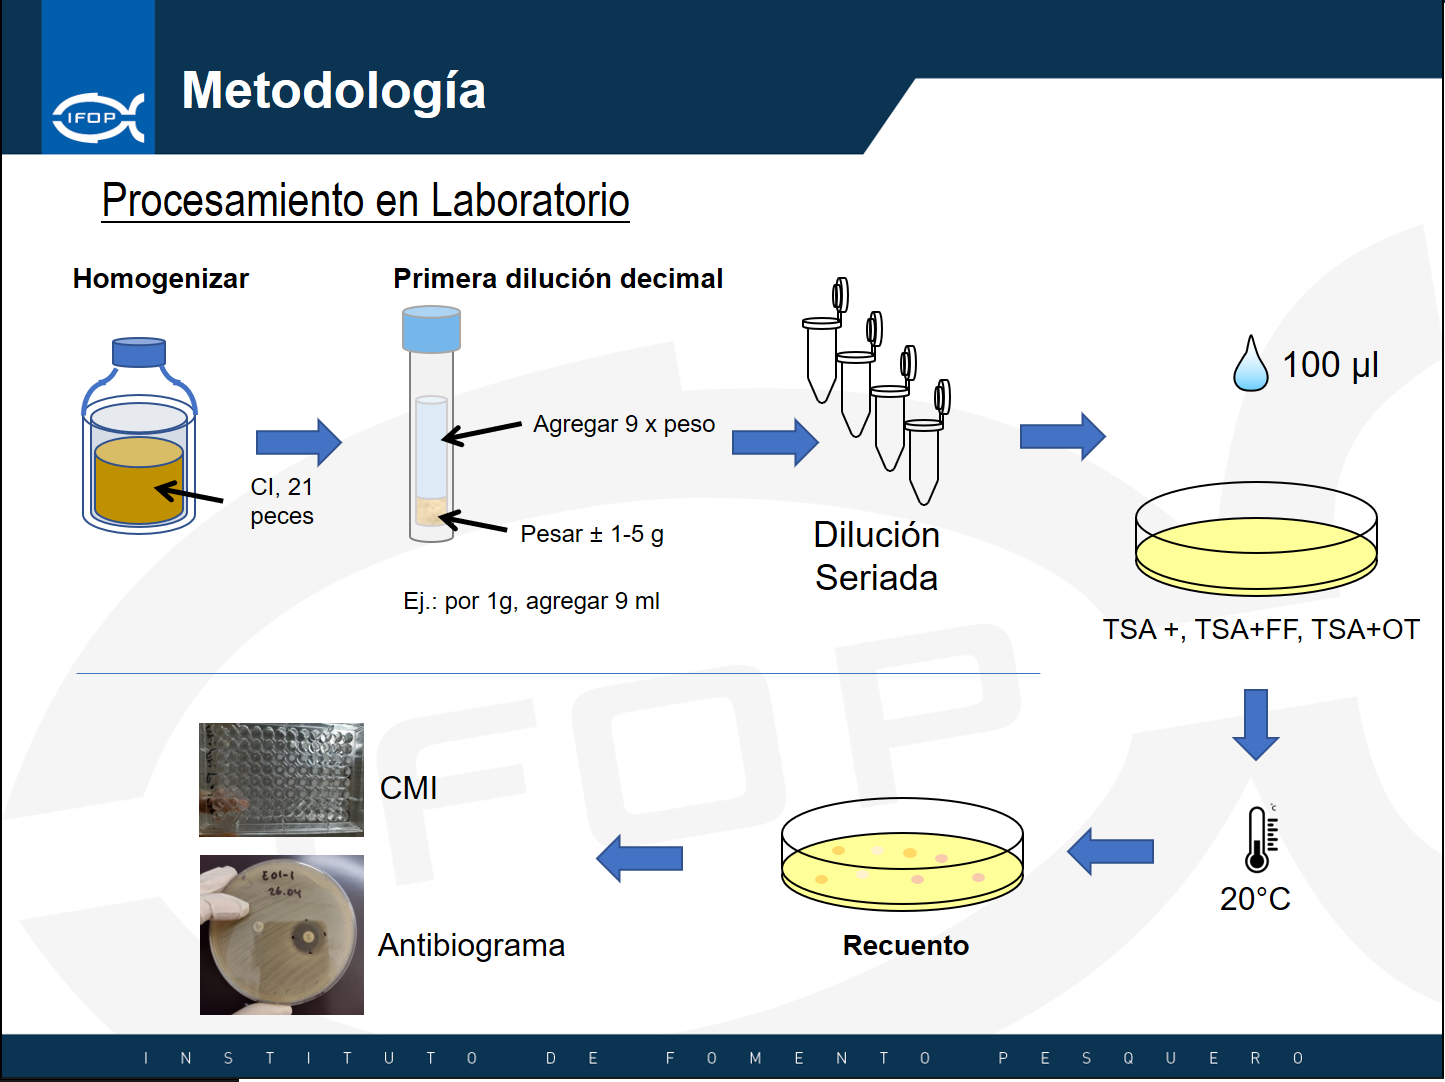
\includegraphics{images/Esquema.png}

}

\end{figure}

\hypertarget{referencia-bibliogruxe1fica}{%
\subsection{Referencia
Bibliográfica}\label{referencia-bibliogruxe1fica}}

Miranda CD. y Rojas R. (2007). Occurrence of florfenicol resistance in
bacteria associated with two Chilean salmon farms with different history
of antibacterial usage. Aquaculture 266, 39--46.



\end{document}
